\chapter{Arquitectura}
\label{chap:arquitectura}

\drop{E}{}ste capítulo analiza en detalle, mediante un enfoque top-down, la arquitectura diseñada para dar soporte al sistema propuesto en este proyecto. Se discutirá la funcionalidad de cada módulo perteneciente a la arquitectura, se explicará cómo están conectados y cómo fluye la información entre ellos hasta obtener el resultado final. 

\section{Visión general de la arquitectura}
\label{sec:visiongeneral}

La arquitectura diseñada (ver Figura~\ref{fig:arquitectura}) es una arquitectura basada en módulos que contribuye a simplificar significativamente el desarrollo del sistema. \\

\begin{figure}[!h]
\begin{center}
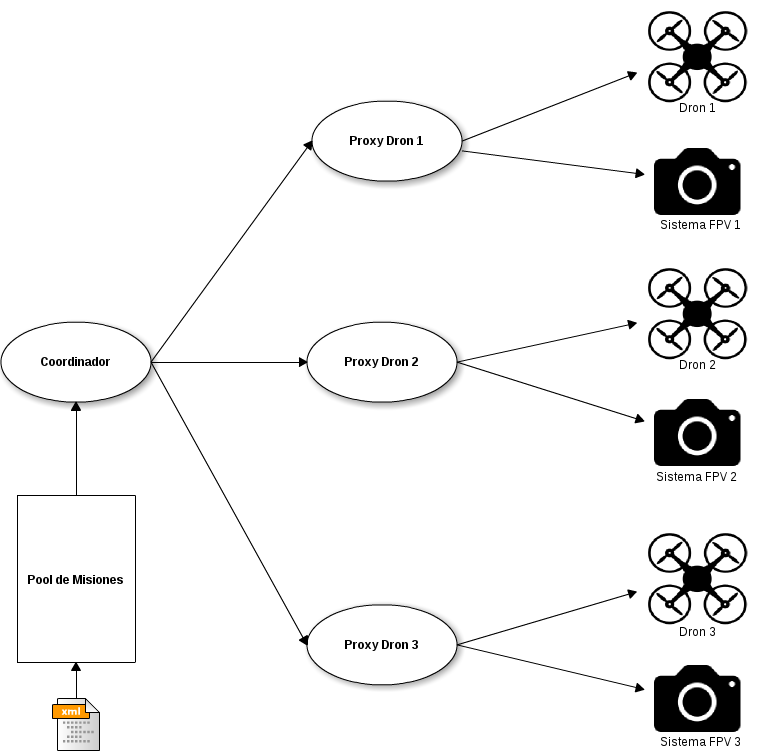
\includegraphics[width=1\textwidth]{/arquitectura.png}
\caption[Arquitectura del sistema]{Arquitectura del sistema}
\label{fig:arquitectura}
\end{center}
\end{figure}

La arquitectura modular se refiere al diseño de sistemas compuestos por elementos separados que pueden conectarse preservando relaciones proporcionales. La utilidad de la arquitectura modular se basa en la posibilidad de reemplazar o agregar cualquier componente sin afectar al resto del sistema.

Al aplicar la arquitectura modular, un problema complejo debe ser dividido en varios subproblemas más simples, y estos a su vez en otros subproblemas más simples. Esto debe hacerse hasta obtener subproblemas lo suficientemente simples como para poder ser resueltos fácilmente con algún lenguaje de programación.

Un módulo es cada una de las partes de un programa que resuelve uno de los subproblemas en que se divide el problema complejo original. Cada uno de estos módulos tiene una tarea bien definida y algunos necesitan de otros para poder operar. En caso de que un módulo necesite de otro, puede comunicarse con éste mediante una interfaz de comunicación que también debe estar bien definida. No debe confundirse el término módulo con términos como función o procedimiento, propios del lenguaje que lo soporte.

En líneas generales, el sistema (ver Figura~\ref{fig:descripcion}) debe ser capaz de extraer «waypoints» de un \textit{Pool de Misiones}, clasificarlos conforme a la prioridad fijada y conseguir que varios drones recorran esos puntos, de forma coordinada, hasta vaciar el \textit{Pool de Misiones}. Así, el sistema reunirá una serie de imágenes, capturadas por los \acs{UAV}s, que deben ser analizadas. \\
 
\begin{figure}[!h]
\begin{center}
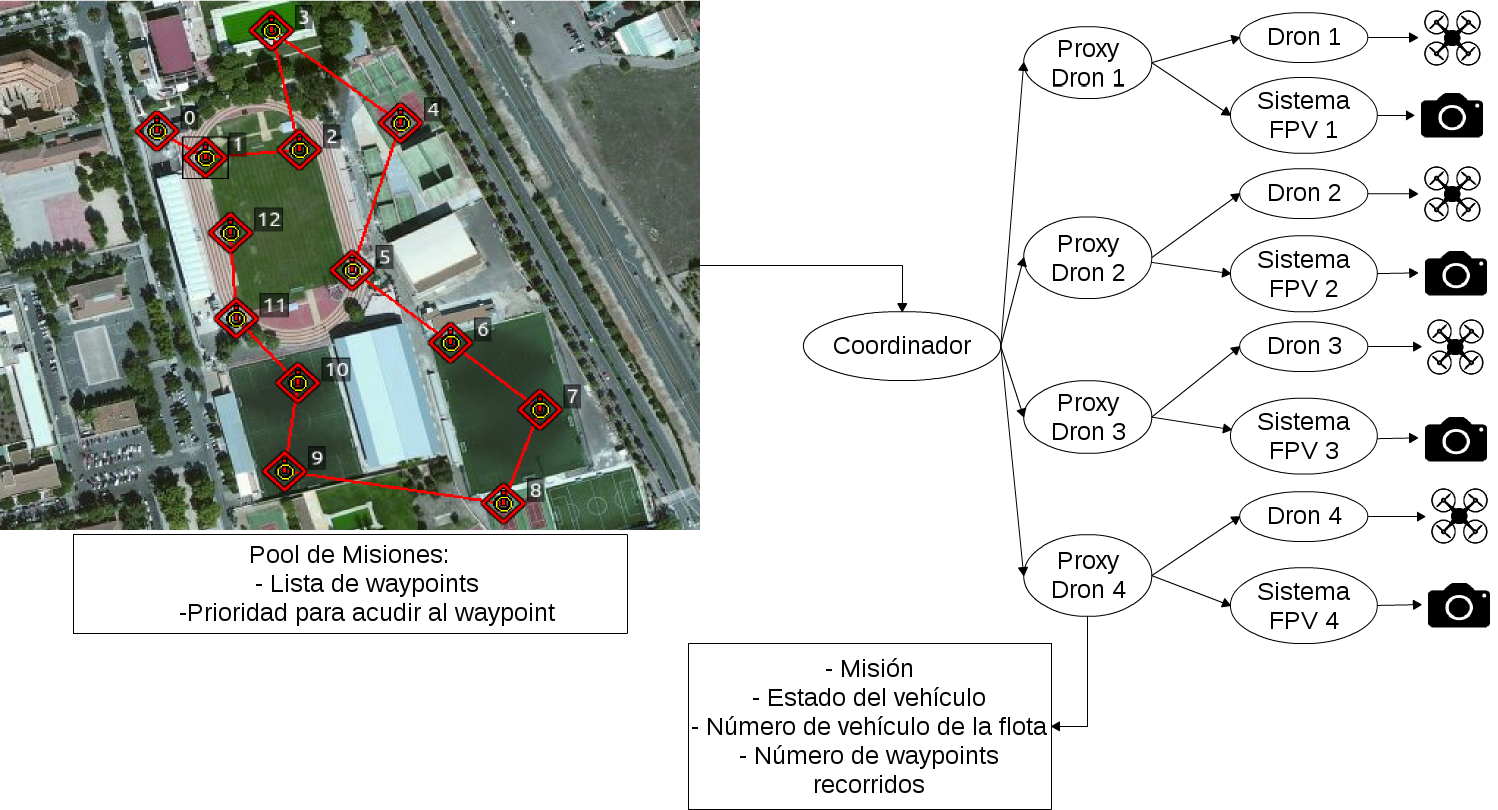
\includegraphics[width=1\textwidth]{/arquitectura2.png}
\caption[Descripción del sistema]{Descripción del sistema}
\label{fig:descripcion}
\end{center}
\end{figure}

En el sistema la información fluye a través de clases (ver Figura~\ref{fig:diagflujo}), transformándose hasta alcanzar el resultado final. Esto es, los vehículos aéreos se desplazan de manera coordinada a diversas localizaciones y a su vez retransmiten imágenes, que son analizadas para contribuir a mejorar los tiempos de respuesta en situaciones de emergencia. \\ \\ \\

\begin{figure}[!h]
\begin{center}
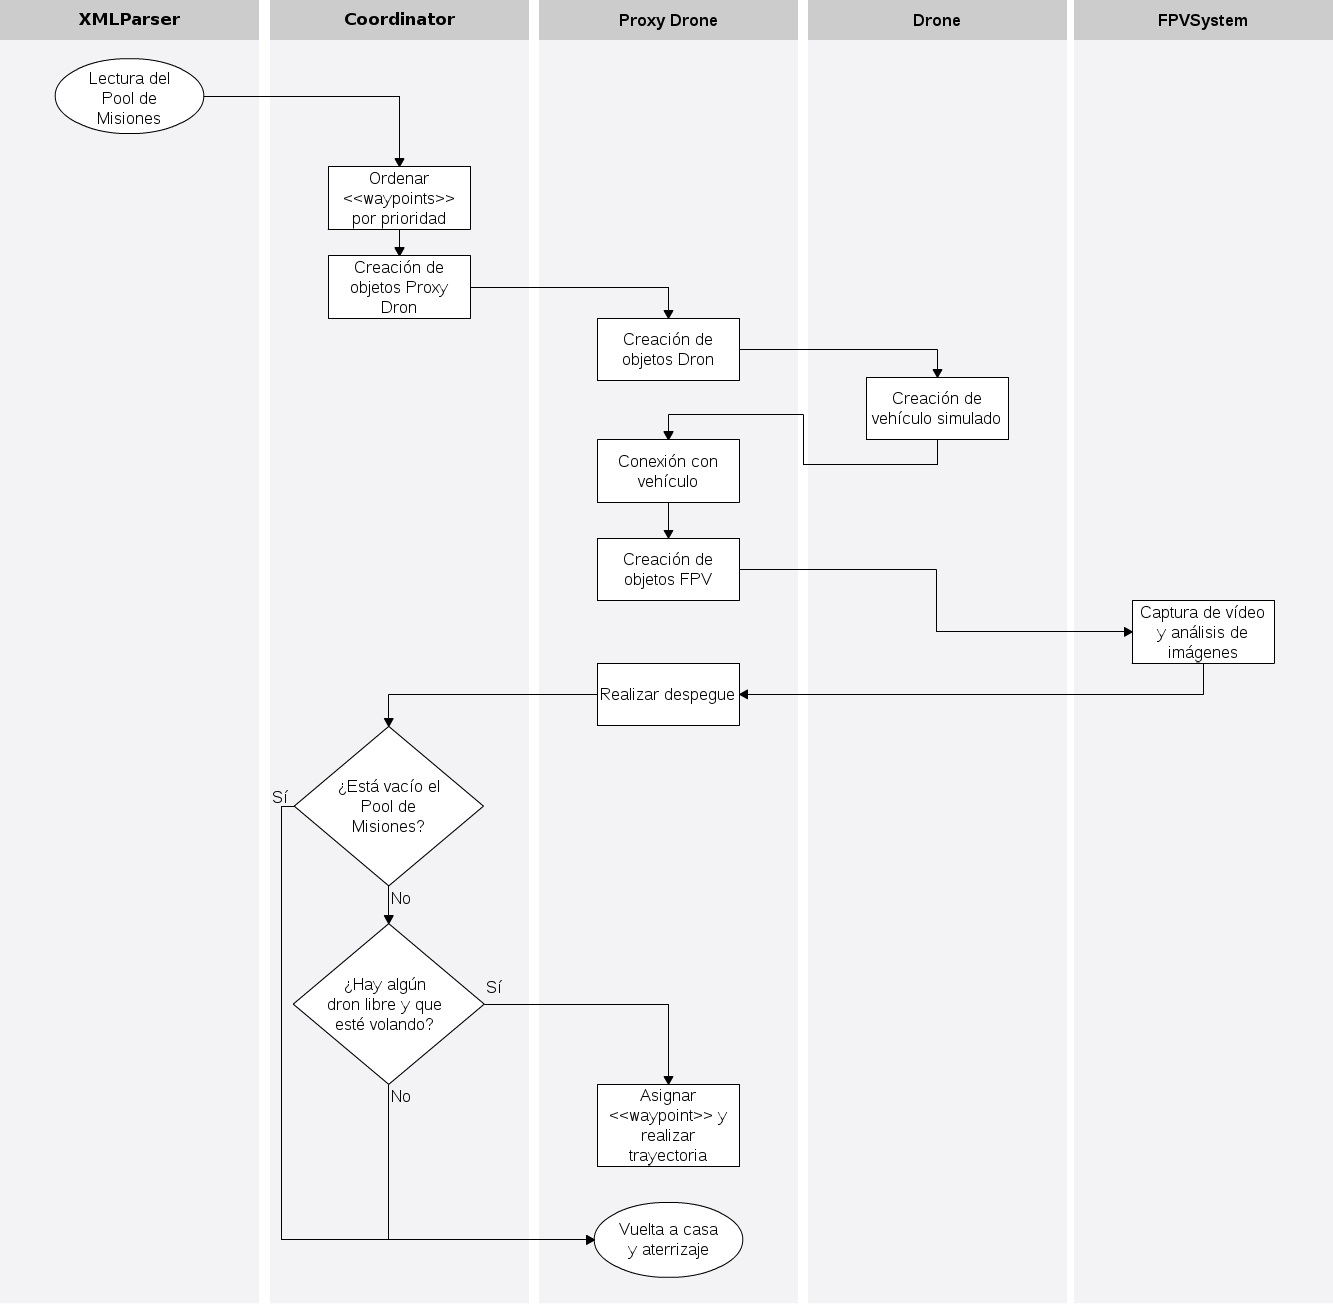
\includegraphics[width=1\textwidth]{/Flowchart.png}
\caption[Diagrama de flujo del sistema con un solo dron]{Diagrama de flujo del sistema con \textbf{un solo dron}}
\label{fig:diagflujo}
\end{center}
\end{figure}

Para ello una iteracción con un solo dron realiza las siguientes tareas:
\begin{itemize}
\item En la clase \textit{XMLParser} se leen los archivos XML, desembocando esto en la \textbf{creación de un \textit{Pool de Misiones}} que contenga todos los puntos que el \acs{UAV} debe monitorizar.
\item El \textit{Coordinator} se encarga de \textbf{ordenar el \textit{Pool de Misiones}} atendiendo a una prioridad extraída de los archivos XML. Además, debe \textbf{crear} tantos \textbf{objetos del tipo \textit{Proxy Drone}} como se hayan especificado, en este caso uno.
\item En la clase \textit{Drone} se obtiene una \textbf{simulación del vehículo aéreo}, a través de \acs{SITL}.
\item Una vez que disponemos de la simulación del dron, se debe realizar la \textbf{conexión con el dron y con el \textit{FPVSystem}}. De esta manera, mientras el \acs{UAV} realiza la misión correspondiente, retransmite imágenes en directo que son analizadas por una \acs{API} externa, \textit{Google Cloud Vision \acs{API}}.
\item Por último, el \textit{Coordinator} debe \textbf{asignar «waypoints»} hasta vaciar el \textit{Pool de Misiones} a drones que se encuentren en estado ocioso.
\end{itemize}

La descripción general de la arquitectura (ver Figura~\ref{fig:arquitectura}) se elaborará a continuación atendiendo al framework y a los módulos que lo componen.

\subsection{Framework}
\label{sec:framework}

Un \textbf{framework} es una estructura conceptual y tecnológica de soporte definido, normalmente con artefactos o módulos concretos de software, que puede servir de base para la organización y desarrollo de software.

En este caso, es el proyecto propuesto, el cual consiste en un sistema de vigilancia adaptativo basado en la coordinación de \acs{UAV}s. Proporciona un conjunto de \textbf{servicios, funciones y herramientas} como puede ser el uso de una estación de control de tierra, la lectura de «waypoints», la ordenación de estos por prioridad o el vuelo de un vehículo aéreo.

\subsection{Módulos desarrollados}
\label{sec:modulos}

Los \textbf{módulos} que se han desarrollado son las unidades básicas que el framework es capaz de manejar y de las que depende la solución que se implemente con él. El sistema está compuesto por los siguientes módulos:

\begin{itemize}
\item \textbf{Módulo de Interpretación de Misiones}: en él se accede a los archivos XML que contienen las referencias de puntos de localización.
\item \textbf{Módulo de Coordinación}: se ordenan esas localizaciones por la prioridad de acudir a cada una de ellas y se coordina la actividad de los drones para mejorar la productividad del sistema. Asigna misiones a vehículos que no estén ejecutando algún vuelo hacia algún «waypoint». Además, ordena el aterrizaje cuando en el \textit{Módulo de Interpretación de Misiones} no queden misiones por asignar.
\item \textbf{Módulo de Despliegue de Alto Nivel}: es el módulo que se conecta y comunica con el vehículo, de modo que, actúa como mediador entre el \textit{Módulo de Coordinación} y el \textit{Módulo de Despliegue de Bajo Nivel}. Permite efectuar tareas relacionadas con el dron, así como administrar la conexión con el \textit{Módulo de Análisis de Información}. Por ejemplo, realizar el despegue de un dron.
\item \textbf{Módulo de Despliegue de Bajo Nivel}: se encarga de crear una simulación de un dron, en una localización específica, para poder realizar pruebas, misiones o cualquier tipo de operación que se podría llevar a cabo con un dron real.
\item \textbf{Módulo de Análisis de Información}: captura, graba y almacena imágenes, en \acs{FPV}, del vuelo del vehículo. Las imágenes son analizadas por una \acs{API} externa de Google, Google Cloud Vision \acs{API}, que detecta conjuntos de categorías y devuelve una serie de resultados después de realizar una petición \acs{HTTP}. 
\end{itemize} 

Cada módulo representa una o más clases (ver Figura~\ref{fig:diagclases}) en las que se define el comportamiento mediante atributos y funciones. Las clases son instanciadas en objetos, que se corresponden tanto con objetos reales como con objetos internos del sistema, en los que se leen estas definiciones.

\begin{figure}[!h]
\begin{center}
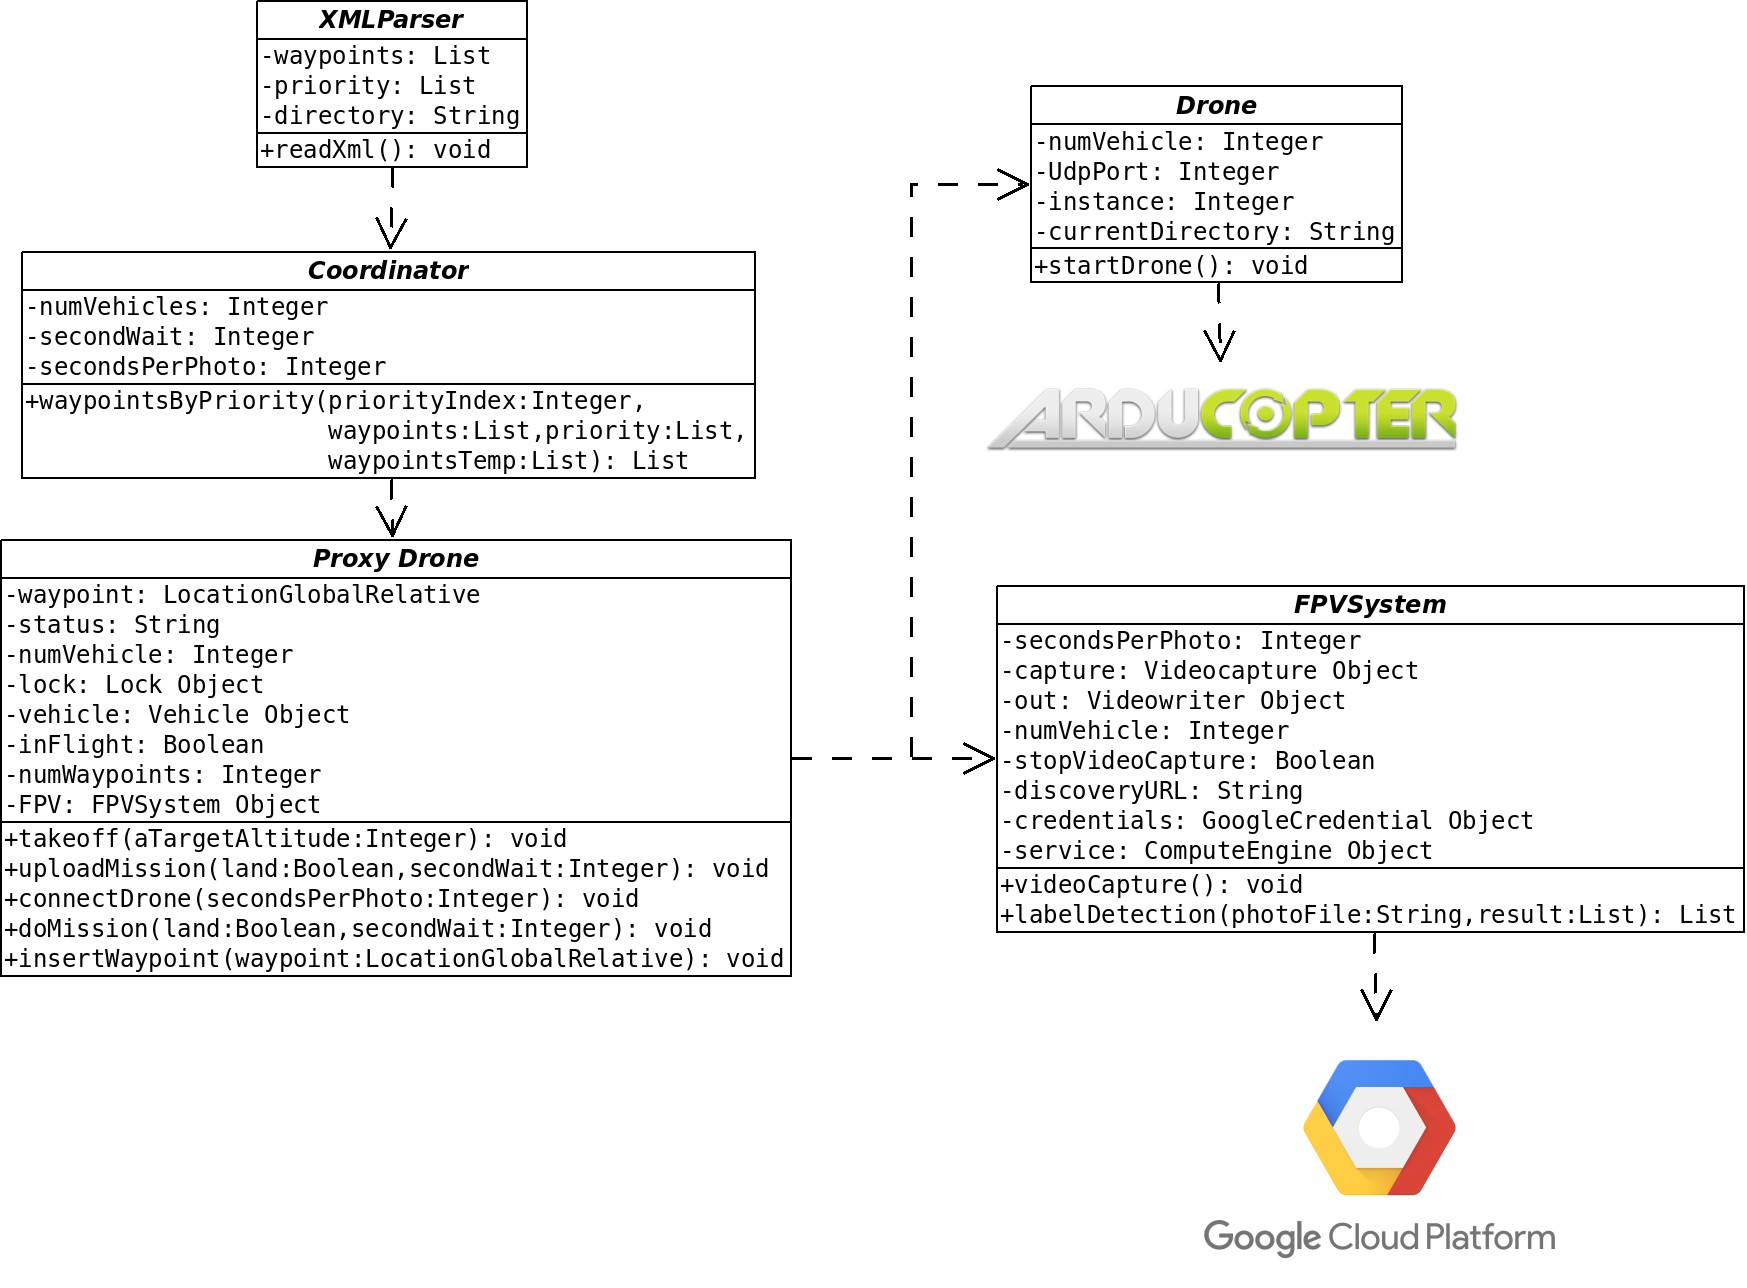
\includegraphics[width=1\textwidth]{/diagclases.png}
\caption[Diagrama de clases del sistema]{Diagrama de clases del sistema}
\label{fig:diagclases}
\end{center}
\end{figure}

El diseño de las clases del sistema se fundamenta en la \textbf{separación de responsabilidades}. La segregación de funciones es un método para separar las responsabilidades de las diversas actividades que intervienen en el sistema, de esta forma, la arquitectura está preparada, por ejemplo, para integrar fácilmente nuevos módulos de análisis a través de otros sensores. También, se debe subrayar que la división entre la clase \textit{Proxy Drone} y las clases \textit{Drone} y \textit{FPVSystem} permite separar las competencias software y hardware, es decir, el \textit{Proxy Drone} se encargará de comunicarse y ordenar tareas a estos dispositivos hardware para así poder cumplir con los objetivos del sistema.

Seguidamente, se expone en detalle cada uno de los módulos desarrollados junto a las clases que forman parte de él.

\section{Módulo de Interpretación de Misiones}

El cometido de este módulo es \textbf{leer los archivos XML}. En esta lectura se recoge la información acerca de los puntos de interés. Esto se realiza con el objetivo de \textbf{crear una estructura de datos}, denominada \textit{Pool de Misiones}, que contenga todo el conocimiento necesario sobre los «waypoints», formados por una ubicación y una prioridad, a los que los drones deben volar durante la misión.


\subsection{Clase XMLParser}

XML es un \textbf{lenguaje de marcas}, desarrollado por el World Wide Web Consortium, utilizado para almacenar datos en forma legible. Permite definir la gramática de lenguajes específicos para estructurar documentos grandes. 

XML se propone como un estándar para el intercambio de información estructurada entre diferentes plataformas. Es una tecnología sencilla que tiene a su alrededor otras que la complementan y la hacen mucho más grande y con unas posibilidades mucho mayores. Tiene un papel muy importante en la actualidad ya que permite la \textbf{compatibilidad entre sistemas para compartir la información} de una manera segura, fiable y fácil. Entre las ventajas que ofrece el uso de XML se encuentran las siguientes:

\begin{itemize}
\item \textbf{Separa} radicalmente \textbf{la información} o el contenido de su presentación o formato.
\item Simplifica compartir e intercambiar datos
\item La información \textbf{se almacena en texto plano}: software y hardware independiente.
\item \textbf{Estructura jerárquica}.
\item Simplifica los cambios de plataforma
\item \textbf{Fácilmente procesable} tanto por humanos como por software.
\end{itemize}

Por esto, se decide hacer uso de archivos XML en los que se especifique la información de los puntos de interés (ver Listado~\ref{code:archivoxml}) que formarán parte de la misión a realizar: \textbf{longitud}, \textbf{latitud}, \textbf{altura} a la que el dron debe volar en dicha posición y la \textbf{prioridad} de que el \acs{UAV} vuele hasta esa localización. 

\begin{listing}[
 float=,
 language = XML,
 caption = {Ejemplo de archivo XML que contiene la información de los «waypoints»},
 label  = code:archivoxml]
<?xml version="1.0" ?>
<mission>
	<waypoint>
 		<lat>-3.9162183</lat>
 		<long>38.9878348</long>
		<alt>30</alt>
		<priority>1</priority>
	</waypoint>

	<waypoint>
 		<lat>-3.9181817</lat>
 		<long>38.9907202</long>
		<alt>25</alt>
		<priority>2</priority>
	</waypoint>

	<waypoint>
 		<lat>-3.9180422</lat>
 		<long>38.9877598</long>
		<alt>20</alt>
		<priority>3</priority>
	</waypoint>
</mission>
\end{listing}

La clase \textit{XMLParser} proporciona una forma de acceder a los datos presentes en los documentos XML. La lectura de estos archivos, que tiene lugar en esta clase, ocasiona la \textbf{creación de una estructura de tipo lista}, que denominaremos \textbf{\textit{Pool de Misiones}}, que contiene una serie de puntos de interés.

\section{Módulo de Coordinación}

Su misión es coordinar la actividad de los drones, durante las misiones, para optimizar la eficiencia del sistema. El cometido de este módulo se divide en tres tareas:

\begin{itemize}
\item \textbf{Ordenar \textit{Pool de Misiones} por prioridad}: con la prioridad que se ha extraído de los archivos XML, se realiza una clasificación del Pool de Misiones, que contiene todos los «waypoints». A causa de esto, las misiones quedarán diseñadas de tal forma que los drones asistan primero a los puntos de interés cuya prioridad sea superior.
\item \textbf{Asignar «waypoints»}: las localizaciones son \textbf{adjudicadas}, hasta vaciar el \textit{Pool de Misiones}, a drones que se encuentren \textbf{\textit{en vuelo}} y que se hallen \textbf{en un \textit{estado ocioso}}, es decir, a drones que ya hayan realizado el despegue y, además, hayan terminado de volar hacia un punto de interés en el que han recogido las imágenes especificadas. 
\item \textbf{Ordenar el aterrizaje}: cuando el \textit{Pool de Misiones} ha sido vaciado, ordenar la vuelta a casa y el aterrizaje de cada uno de los drones que se estaban empleando en el proceso.
\end{itemize}

\subsection{Clase Coordinator}

El \textit{Coordinator} es el responsable de llevar a cabo la \textbf{coordinación}, \textbf{entre los \acs{UAV}s} que existan disponibles, con el objetivo de poder abarcar el mayor terreno posible en un tiempo que es considerablemente menor. Para llevar a cabo este propósito es necesario contar antes con un \textit{Pool de Misiones} que se encuentre ordenado por la prioridad de los «waypoints». 

Una vez que los archivos XML han sido leídos y los «waypoints» han sido almacenados en el \textit{Pool de Misiones}, el \textit{Coordinator} debe \textbf{ordenar} esas localizaciones \textbf{por medio del campo prioridad}. La prioridad puede tomar tres valores diferentes: 1, 2 y 3. Siendo 1 la prioridad más elevada y 3 la de menor relevancia. De modo que, en el \textit{Pool de Misiones} deben aparecer primero los  cuya prioridad sea de 1 y en último lugar los que tengan una prioridad de 3, consiguiendo que los drones lleguen antes a los puntos de interés más importantes.

Con el \textit{Pool de Misiones} ordenado, el \textit{Coordinator} comenzará a asignar «waypoints» a drones que ya hayan realizado el despegue y no se encuentren volando hacia algún otro punto de interés. Cuando el \textit{Pool de Misiones} se encuentre vacío, el \textit{Coordinator} dará la orden de aterrizaje a los drones existentes.

Es crucial que varios drones puedan \textbf{efectuar a la vez el vuelo y la captura de vídeo}, por lo que es necesario la \textbf{introducción de hilos} en el \textit{Coordinator}, que permitan ejecutar, de manera paralela, estas funciones. 

La técnica de multi-hilos permite \textbf{desacoplar tareas que no tienen dependencia secuencial}. El trabajo con threads se lleva a cabo mediante el \textbf{módulo \textit{threading}} que se apoya en el módulo \textit{thread} para proporcionar una \acs{API} de más alto nivel, más completa y orientada a objetos. 

El desafío principal de las aplicaciones multi-hilo es la coordinación entre los hilos que comparten datos u otros recursos. Con ese fin, el módulo \textit{threading} provee una serie de primitivas de sincronización que incluyen \textbf{\textit{locks}}, eventos, variables de condición y semáforos. 

Los \textit{locks}, también llamados mutex, cierres de exclusión mutua, cierres o candados, son objetos con \textbf{dos estados posibles: adquirido o libre}. Cuando un \textit{thread} adquiere el candado, los demás \textit{thread} que lleguen a ese punto posteriormente y pidan adquirirlo se bloquearán hasta que el \textit{thread} que lo ha adquirido libere el candado, momento en el cual podrá entrar otro \textit{thread}.

Para iniciar el sistema, se debe realizar una llamada a la clase \textbf{\textit{Coordinator}}, la cual cuenta con tres argumentos que son parametrizables al realizar su invocación por consola. Estos atributos parametrizables son los siguientes:
\begin{itemize}
\item \textbf{numVehicles}: se refiere al número de vehículos que participarán en las misiones y capturarán imágenes en directo del vuelo. Si se omite, el valor por defecto es 1 vehículo.
\item \textbf{secondWait}: afecta al número de segundos que el vehículo permanecerá parado sobre un «waypoint» para captar imágenes relevantes de esa localización durante ese tiempo. Si se omite, el valor por defecto es de 10 segundos.
\item \textbf{secondsPerPhoto}: referido al número de segundos que deben transcurrir para tomar una fotografía. Por ejemplo, si el valor es de 5 segundos, el sistema realizará una fotografía cada 5 segundos. Si se omite, el valor por defecto es de 10 segundos.
\end{itemize} 

Un ejemplo de cómo realizar la llamada a \textit{Coordinator} puede ser:

\begin{listing}[
 float=h!,
 language = bash,
 caption = {Ejemplo de llamada a \textit{Coordinator}},
 label  = code:coordinador]
$ python coordinator.py --vehicles 2 --secondWait 15 --secondsPerPhoto 7
\end{listing}

Para conseguir que el sistema funcione, es necesaria la instalación de varias dependencias. Se pueden consultar en el Anexo \ref{chap:dependencias}.

\section{Módulo de Despliegue de Alto Nivel}

Es el módulo responsable a la hora de realizar las operaciones que conciernen al vehículo, como el despegue o la subida de misiones, y de gestionar la conexión con los dispositivos finales, como el \textbf{dron} o el \textbf{sistema \acs{FPV}}. Actúa de intermediario entre el \textit{Módulo de Coordinación} y los módulos de \textit{Despliegue de Bajo Nivel} y de \textit{Análisis de Información}.
\subsection{Clase Proxy Drone}

El \textbf{\textit{Proxy Drone}} es el encargado de ejecutar las tareas que tienen que ver con el \acs{UAV} y de administrar la conexión con los dispositivos finales. Se puede considerar un \textbf{intermediario} entre el \textit{Coordinator} y los instrumentos que se encuentran en el extremo del sistema, \textit{Drone} y \textit{FPVSystem}, que son usados para realizar el vuelo y captar imágenes.

Mediante el \textit{Proxy Drone} se resuelve el problema de \textbf{guiar el vehículo} a través de una serie de puntos de localización. Gracias a él, el sistema cuenta con una clase que posibilita la \textbf{comunicación con el dron} y el \textbf{visionado en primera persona}, permitiendo así realizar cualquier tipo de operación como el despegue, la asignación de puntos de interés, la realización de vuelos a dichos puntos o la captación de imágenes que puedan ayudar al personal de emergencia en las labores de identificación de supervivientes o inspección del terreno.

Tan pronto como se haya realizado la lectura de los archivos XML y se cuente con una lista de «waypoints» ordenados por prioridad, se procede a crear objetos de tipo \textbf{\textit{Proxy Drone}}. 
Para ello, el \textit{Coordinator} hace uso de su atributo \textit{numVehicles}, creando tantos objetos \textit{Proxy Drone} como número de vehículos se haya especificado.

Entre las competencias de esta clase se encuentran las que se exponen a continuación:

\begin{itemize}
\item \textbf{Conexión con el dron} y con el \textbf{Sistema \acs{FPV}}: En el caso de ejecutar una simulación del sistema, se instancia un objeto de tipo \textit{Drone}, que creará un vehículo simulado mediante \acs{SITL} (véase Sección \ref{sec:sitl}). A continuación, se realiza la conexión con el vehículo aéreo, ya sea real o simulado, y por último se crea un objeto \textit{FPVSystem} para iniciar la grabación y el análisis de imágenes.
\item \textbf{Despegue} del dron: se comprueba que el vehículo cumpla ciertos requisitos antes de armar los motores, como que disponga de una buena señal de \acs{GPS} o que el nivel de la batería sea superior al 50\%, se configura el modo de pilotaje del dron y se procede al despegue a una altura especificada por parámetro. Cuando el despegue ha terminado, el dron se considera \textit{en vuelo}. 
\item \textbf{Inserción de «waypoints»} y \textbf{escritura de misiones}: los «waypoints», que han sido extraídos del archivo XML en el \textit{Coordinator}, son adjudicados a drones que se encuentren en \textit{estado ocioso} y \textit{en vuelo}. La localización de estos puntos debe ser agregada a comandos de misión que puedan ser interpretados por el vehículo. Entre estos comandos se encuentran las órdenes necesarias para: acudir a una localización específica, mantener el vehículo en un punto concreto o realizar la vuelta a casa y el aterrizaje.
\end{itemize}

El \textit{Proxy Drone} es inicializado pasándole por parámetro el número de vehículo con el que se corresponde dicho objeto. Gracias a esto, el usuario puede obtener \textbf{información del estado del dron}, sabiendo, por ejemplo, si esa información está asociada al \textit{Dron 1} o al \textit{Dron 2}.

\clearpage

\section{Módulo de Despliegue de Bajo Nivel}

Se ocupa de generar una simulación de un \acs{UAV}, en una ubicación determinada, de modo que se puedan realizar pruebas, misiones o cualquier tipo de operación sin tener que disponer de un vehículo real.

\subsection{Clase Drone}

La clase \textbf{\textit{Drone}} ofrece la posibilidad de \textbf{simular vehículos aéreos} (ver Figura~\ref{fig:dronSITL}), en el caso de este proyecto un quadcopter, haciendo uso de la aplicación \acs{SITL}.

\begin{figure}[!h]
\begin{center}
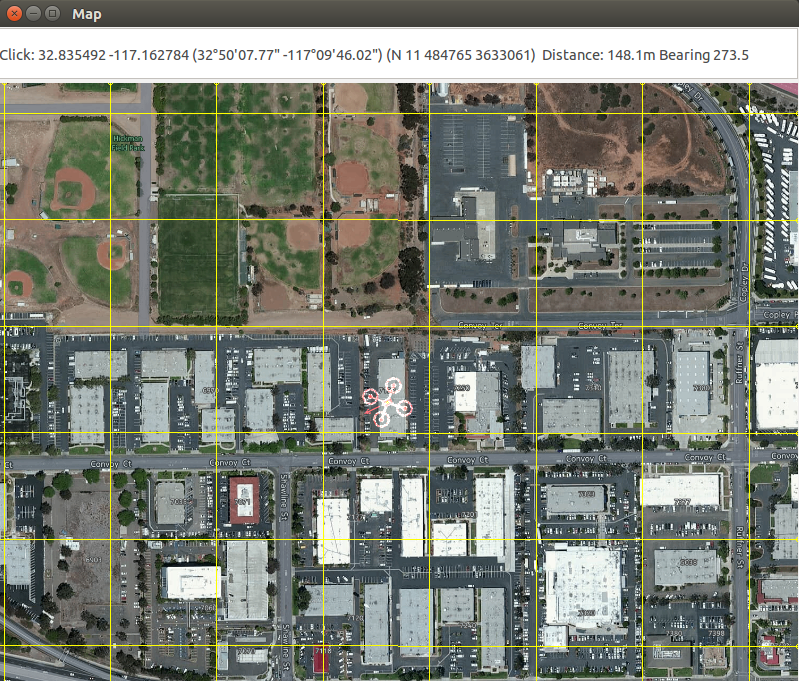
\includegraphics[width=0.8\textwidth]{/dronSITL.png}
\caption[Simulación de dron mediante \acs{SITL}]{Simulación de dron mediante \acs{SITL}}
\label{fig:dronSITL}
\end{center}
\end{figure}

El uso de \acs{SITL} (véase Sección \ref{sec:sitl}) permite crear vehículos simulados que pueden usarse como un vehículo real: se puede conectar al vehículo usando una estación de control de tierra, despegar, cambiar los modos de vuelo, realizar misiones guiadas o automáticas, y aterrizar. La diferencia principal es que además de ser capaz de configurar el vehículo, los parámetros del simulador permiten configurar el entorno físico (por ejemplo, la velocidad y dirección del viento) y también simular el fallo de distintos componentes. Esto significa que \acs{SITL} es el entorno perfecto para probar correcciones de errores y otros cambios en el piloto automático, modos de fallo y aplicaciones desarrolladas mediante DroneKit-Python (véase Sección \ref{sec:dronekit}).

\clearpage

El cometido que tiene esta clase es, dependiendo del número de vehículo que lo instancie, acceder a una carpeta determinada y \textbf{ejecutar el comando} (ver Listado~\ref{code:simulacion}) \textbf{para generar la simulación} del dron, en un puerto UDP concreto, al que posteriormente el sistema se conectará para comunicarse con él.

\begin{listing}[
 float=h!,
 language = bash,
 caption = {Comando para generar una simulación de un vehículo mediante \acs{SITL}},
 label  = code:simulacion]
$ sim_vehicle.sh -I %d -L prueba --map --out 127.0.0.1:%d --aircraft test
\end{listing}

El comando está formado por unos parámetros que representan lo siguiente:
\begin{itemize}
\item \textbf{-I}: el número de instancia para permitir múltiples copias del simulador funcionando a la vez.
\item \textbf{-L}: ubicación inicial, que es configurada en un archivo de tipo texto denominado \textit{locations.txt}.
\item \textbf{$-$$-$map}: posibilita disponer de una ventana con un mapa, para mostrar el progreso del dron al realizar las misiones.
\item \textbf{$-$$-$out}: dirección en la que se podrá realizar la conexión con el dron. Está formada por una dirección IP y un puerto UDP.
\end{itemize}

\section{Módulo de Análisis de Información}

Capta, registra y guarda imágenes de vídeo del vuelo del vehículo. Realiza capturas de pantalla, del vídeo en \acs{FPV}, que son analizadas por Google Cloud Vision \acs{API}, que es capaz de detectar grupos de categorías y retornar una cadena de resultados.

\subsection{Clase FPVSystem}

Los objetos de la clase \textbf{\textit{FPVSystem}} facilitan la captura de imágenes en \acs{FPV} y el análisis de estas.

Las tareas que se desarrollan en esta clase son fundamentalmente tres:
\begin{itemize}
\item \textbf{Grabación de vídeo}: el sistema graba y almacena un vídeo, haciendo uso de \textit{OpenCV} (véase Sección \ref{sec:opencv}), que facilitará a los equipos de emergencia la visión del terreno, para así, poder tomar unas decisiones mejores y más correctas.
\item Realización de \textbf{captura de pantalla}: cada un cierto número de segundos, especificado al realizar la llamada al \textit{Coordinator}, se llevará a cabo una captura de pantalla que será almacenada en el computador y que será utilizada para realizar el análisis.
\item \textbf{Análisis de imágenes}: haciendo uso de Google Cloud Vision \acs{API} (véase Sección \ref{sec:visionapi}) se analizarán las capturas de pantalla realizadas anteriormente. Google Cloud Vision \acs{API}, mediante la detección de etiquetas, detecta amplios conjuntos de categorías y arroja resultados de los elementos que se encuentran dentro de las fotografías. Estos resultados serán imprimidos y mostrados en el vídeo que se está grabando.
\end{itemize}

Para llevar a cabo el análisis de imágenes es necesario realizar una \textbf{petición \acs{HTTP} a Google Cloud Vision \acs{API}} en la que se especifique el tipo de análisis que se quiere realizar, en este supuesto \textit{Detección de etiquetas}, y el número máximo de resultados a obtener.

Un ejemplo de esta petición puede ser la especificada a continuación:

\begin{listing}[
 float=h!,
 language = Python,
 caption = {Ejemplo de petición a Google Cloud Vision \acs{API} para la detección de etiquetas},
 label  = code:analisis]
with open(photoFile, 'rb') as image:
	image_content = base64.b64encode(image.read())
    service_request = self.service.images().annotate(body = {
    	'requests': [{
        	'image': {
          		'content': image_content.decode('UTF-8')
        			},
        		'features': [{
          			'type': 'LABEL_DETECTION',
          			'maxResults': 5
        		}]
      	}]
    }]
    
		
    response = service_request.execute()
	responseLength = len(response['responses'][0])
\end{listing}

Haciendo uso de dicha función, se obtiene el análisis de una imagen que arroja como resultado cinco etiquetas.  

\begin{figure}[!h]
\begin{center}
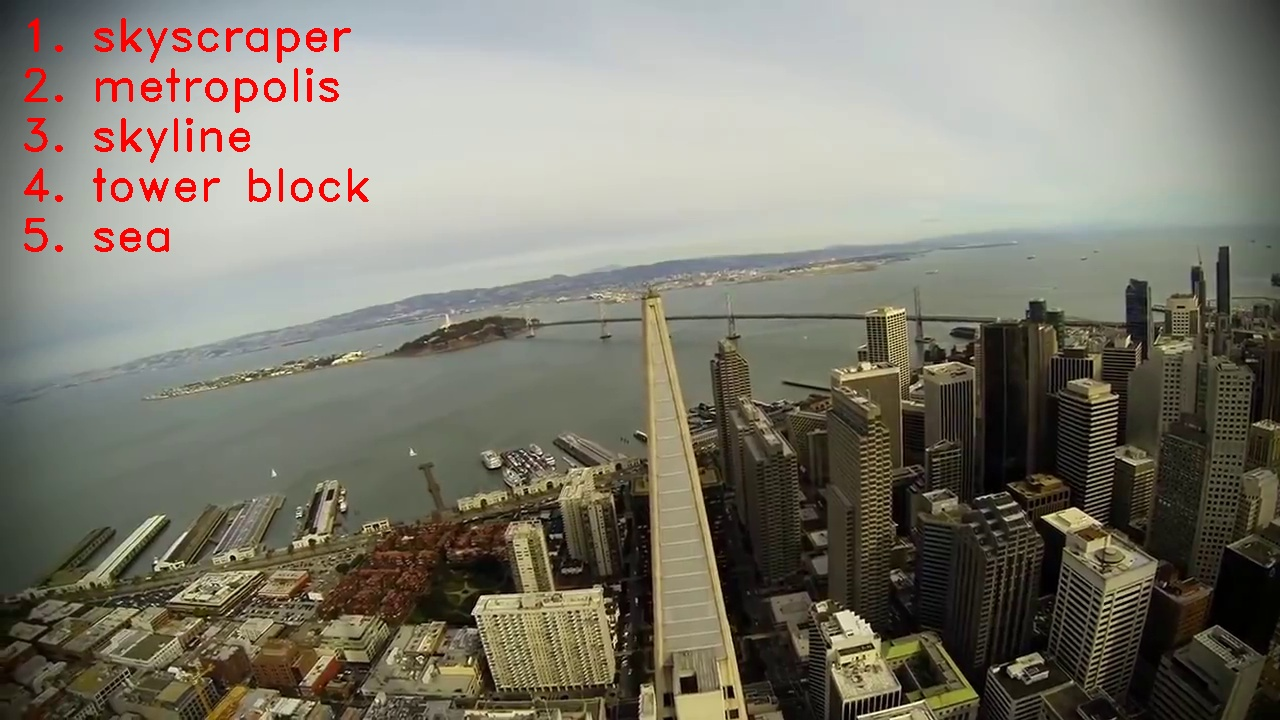
\includegraphics[width=0.8\textwidth]{/ejemplofpv.jpg}
\caption[Ejemplo de captura y análisis de imagen]{Ejemplo de captura y análisis de imagen}
\label{fig:ejemplofpv}
\end{center}
\end{figure}

% Local Variables:
% coding: utf-8
% mode: latex
% mode: flyspell
% ispell-local-dictionary: "castellano8"
% End:
